\documentclass[border=10pt]{standalone}

\usepackage{tikz}
\usepackage{tikzsymbols}
\usetikzlibrary{calc,patterns,shapes.geometric}

\def\centerarc[#1](#2)(#3:#4:#5){\draw[#1] ($(#2)+({#5*cos(#3)},{#5*sin(#3)})$) arc (#3:#4:#5);}

\begin{document}
	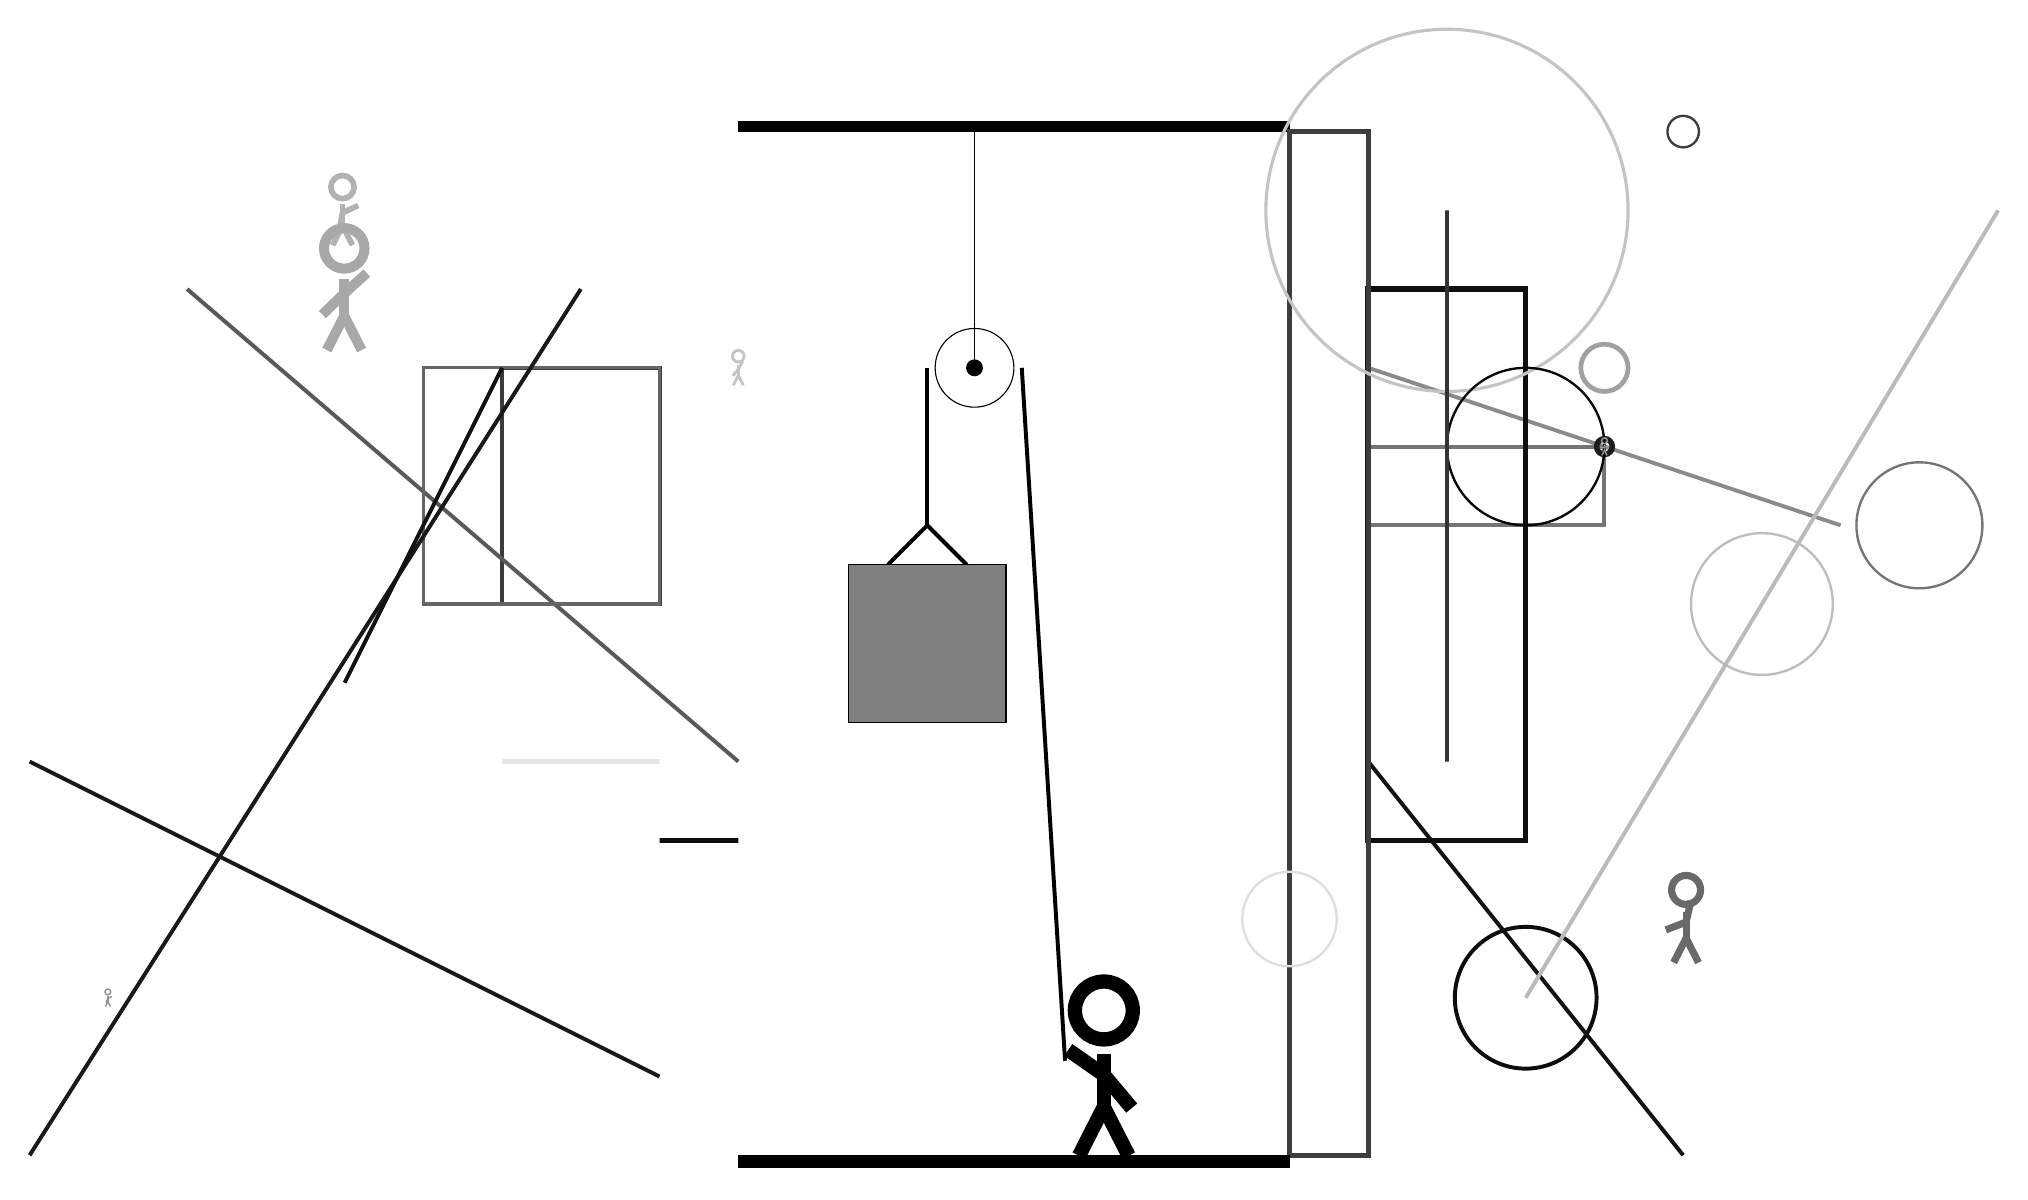
\begin{tikzpicture}
		%%%%% START %%%%%
		
		\draw[fill=black] (-2, 10) rectangle (5, 10.125);
		
		\draw (1, 7) circle (0.5);
		\draw[fill=black] (1, 7) circle (0.1);
		\draw (1, 10) -- (1, 7);
		
		\draw[line width=0.5mm] (-0.1, 4.5) -- (0.4, 5.0) -- (0.9, 4.5);
		\draw[fill=black!50] (-0.6, 4.5) rectangle (1.4, 2.5);
		
		\draw [line width=0.3mm, color=black!26](11, 4) circle (0.9);
		
		\draw[line width=0.5mm, color=black!46](6, 7) -- (12, 5);
		\draw [line width=0.5mm, color=black!95](8, -1) circle (0.9);
		\draw[line width=0.7mm, color=black!10] (-3, 2) rectangle (-5, 2);
		\node[line width=0.2mm, color=black!30] at (-7, 9) {\Strichmaxerl[4][79][25]};
		\draw[line width=0.5mm, color=black!90](-3, -2) -- (-11, 2);
		
		\draw[line width=0.5mm, color=black!87](5, 0) -- (5, 6);
		
		\draw[line width=0.5mm, color=black!54] (6, 6) rectangle (9, 5);
		\draw[line width=0.5mm, color=black!77] (-3, 4) rectangle (-5, 7);
		
		\draw[line width=0.5mm, color=black!93](10, -3) -- (6, 2);
		\node[line width=0.3mm, color=black!43] at (-10, -1) {\Strichmaxerl[1][67][24]};
		
		\draw[line width=0.7mm, color=black!94] (6, 8) rectangle (8, 1);
		\draw[line width=0.5mm, color=black!65](-2, 2) -- (-9, 8);
		
		\draw [line width=0.7mm, color=black!89](9, 6) circle (0.1);
		\draw[line width=0.5mm, color=black!27](8, -1) -- (14, 9);
		\draw [line width=0.6mm, color=black!37](9, 7) circle (0.3);
		\draw[line width=0.6mm, color=black!76] (6, 10) rectangle (5, -3);
		\node[line width=0.7mm, color=black!34] at (-7, 8) {\Strichmaxerl[7][44][42]};
		\draw [line width=0.3mm, color=black!13](5, 0) circle (0.6);
		\draw [line width=0.4mm, color=black!23](7, 9) circle (2.3);
		\node[line width=0.4mm, color=black!59] at (10, 0) {\Strichmaxerl[5][21][77]};
		
		\draw [line width=0.3mm, color=black!97](8, 6) circle (1.0);
		\draw[line width=0.7mm, color=black!95] (-3, 1) rectangle (-2, 1);
		\draw[line width=0.6mm, color=black!80] (7, 9) rectangle (7, 2);
		\draw [line width=0.3mm, color=black!54](13, 5) circle (0.8);
		\draw [line width=0.3mm, color=black!76](10, 10) circle (0.2);
		\draw[line width=0.4mm, color=black!60] (-3, 4) rectangle (-6, 7);
		\draw[line width=0.5mm, color=black!90](-4, 8) -- (-11, -3);
		\node[line width=0.6mm, color=black!23] at (-2, 7) {\Strichmaxerl[2][52][60]};
		\draw[line width=0.5mm, color=black!93](-7, 3) -- (-5, 7);
		\node[line width=0.5mm, color=black!41] at (9, 6) {\Strichmaxerl[1][10][19]};
		
		
		\draw[line width=0.5mm] (0.4, 7) -- (0.4, 5.0);
		\centerarc[line width=0.5mm](1, 7)(0:180:0.6);
		\draw[line width=0.5mm](1.6, 7) -- (2.15, -1.8);
		
		\node at (2.6, -1.9) {\Strichmaxerl[10][-35][-50]};
		
		\draw[fill=black] (-2, -3) rectangle (5, -3.15);
		
		%%%%% END %%%%%
	\end{tikzpicture}
\end{document}